\documentclass[a4paper,12pt]{report}
\usepackage{graphicx}
\usepackage{titlesec}
\titleformat{\chapter}{}{}{0em}{\bf\LARGE}
\usepackage[utf8]{inputenc}

% Title Page
\title{Middle East Technical University\\Department of Physics\\PHYS222 Optics and Waves Laboratory\\\textbf{Experiment OW-2 Prism Spectrometer\\Laboratory Report}}

\author{Oğuzhan ÖZCAN\\1852334\\\\Partner: İnci SAİM\\\\Teaching Assistant: Hikmet ÖZŞAHİN}


\begin{document}
\maketitle
\tableofcontents
\listoffigures
\listoftables
\chapter{Theory}
A prism spectrometer is a device where the light is dispersed by a prism. This optical element disperses parallel rays or collimated radiation into different angles from the prism. An ordinary spectrometer consists of a light source, a collimator with a slit, a prism which is located at middle of table, and an eye piece (See Figure 1.1). In this sense wavelength and index are very important because angle of deviation is depends on these quantities. The angle of deviation is shown by $\delta$ and angle of minimum daviation is shown by $\delta_{m}$$[1]$. Angle of deviation can be calculated by using \begin{center}
{\large 	$\delta=\theta_{2}^{\prime}+\omega$}
\end{center}  
or instead of using $\omega$ we can use angle $\alpha$ which is formed by the edge of prism (See Figure 1.2).
\begin{center}
{\large 	$\delta=\theta_{1}+\theta_{2}^{\prime}+\alpha$}
\end{center}
\begin{figure}[h]
\centering
\includegraphics[width=0.7\linewidth, height=0.25\textheight]{"prism spectrometer"}
\caption{Prism Spectrometer}
\label{fig:prismspectrometer}
\end{figure}
Angle of minimum deviation $\delta_{m}$ is formed by the angle of incidence $\theta_{1}$. When the angle of incidence $\theta_{1}$ is varied from an arbitrary point, the deviation angle $\delta$ will become smaller until it reaches a minimum point. This variation can be caused by either rotating the prism or moving the light source.
\newpage
\begin{figure}
\centering
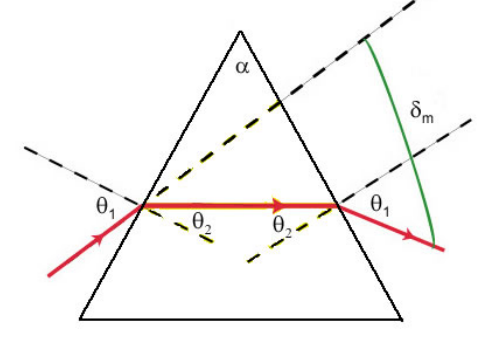
\includegraphics[width=0.30\linewidth, height=0.17\textheight]{dispersion}
\caption{Prism Dispersion}
\label{fig:dispersion}
\end{figure}

When we make further calculations we will get some important quantities such as index of prism and relation between index \textit{n} and minimum angle of deviation $\delta_{m}$. For the minimum angle of deviation $\delta_{m}$ following equaitons should be satisfied;
\begin{center}
	{\large $n_{s}\sin\theta_{1}=n_{p}\sin\theta_{1}^{\prime}$}
\end{center}
\begin{center}
	 {\large $\theta_{1}^{\prime}=\theta_{2}=\frac{\alpha}{2}$ and $\theta_{1}=\theta_{2}^{\prime}=\frac{\alpha+\delta_{m}}{2}$}
\end{center}
When the index of refraction of air to be $n_{s}=1.00$
\begin{center}
{\large 	$1.00\sin[\frac{\alpha+\delta_{m}}{2}]=n_{p}\sin[\frac{\alpha}{2}]$}
\end{center}
and when we insert $\theta_{1}$ and $\theta_{2}$ into Snell's law, this manipulation gives a simple equation for the index of refraction of the prism $[2]$,
\begin{center}
	{\Large $n_{p}=\frac{\sin[\frac{\alpha+\delta_{m}}{2}]}{\sin[\frac{\alpha}{2}]}$}
\end{center}
In a despersive material, the index of refraction depends on the wavelength $\lambda$ of the incident light $[3]$. When we write the index of refraction of the prism in terms of wavelength, we get   
\begin{center}
	{\Large $n(\lambda)=\frac{\sin[\frac{\alpha+\delta_{m}(\lambda)}{2}]}{\sin[\frac{\alpha}{2}]}$}
\end{center}
Obviously the index of refraction is not same for all wavelengths or colors. As we can see from previous equation the index of refraction of prism depends on the wavelength of the incident light. We can see this relationship with \textit{Cauchy's formula} $[4]$,
\begin{center}
	{\Large $n=A+\frac{B}{\lambda^{2}}+\frac{C}{\lambda^{4}}$}
\end{center}
where \textit{A, B} and \textit{C} are called Cauchy's constants.
















\chapter{Data and Results}
\begin{table}[h]
\begin{center}
	\begin{tabular}{|c|c|c|}
	\hline Position 1 & Position 2 & $\alpha_{i}$ \\ 
	\hline $61^{\circ}28^{\prime}$ & $301^{\circ}8^{\prime}$ & $59^{\circ}46^{\prime}$ \\ 
	\hline $57^{\circ}7^{\prime}$ & $296^{\circ}21^{\prime}$ & $59^{\circ}40^{\prime}$ \\ 
	\hline $65^{\circ}10^{\prime}$ & $305^{\circ}12^{\prime}$ & $59^{\circ}39^{\prime}$ \\ 
	\hline 
\end{tabular} 
\end{center}
\caption{Data for the Prism Angle $\alpha$}
\end{table}
To find the average $\alpha_{i}$;
\begin{center}
	$\bar{a}=\frac{\alpha_{1}+\alpha_{2}+\alpha_{3}}{3}$ \\$\bar{a}=59^{\circ}42^{\prime}$
\end{center}



\begin{table}[h]
\begin{center}
	\begin{tabular}{|c|c|c|c|c|}
	\hline $\lambda$ & Position 1 & Position 2 & $\delta_{min}$ & n \\ 
	\hline Violet & $1^{\circ}30^{\prime}$ & $38^{\circ}52^{\prime}$ & $48^{\circ}44^{\prime}$ & 1.562 \\ 
	\hline Blue & $1^{\circ}30^{\prime}$ & $40^{\circ}46^{\prime}$ & $48^{\circ}35^{\prime}$ & 1.558 \\ 
	\hline Green & $1^{\circ}30^{\prime}$ & $31^{\circ}48^{\prime}$ & $48^{\circ}19^{\prime}$ & 1.552 \\ 
	\hline Orange & $1^{\circ}30^{\prime}$ & $36^{\circ}43^{\prime}$ & $47^{\circ}52^{\prime}$ & 1.549 \\ 
	\hline 
\end{tabular} 
\end{center}
\caption{Data for the Refractive Index versus Wavelength}
\end{table}
To define the related refractive index for each color we are going to use the following formula;
\begin{center}
	{\large $n=\frac{\sin(\frac{\alpha+\delta_{min}}{2})}{\sin\frac{\alpha}{2}}$}
\end{center}
for $\lambda_{violet}$
\begin{center}
{\large 	$n=\frac{\sin(\frac{59^{\circ}42^{\prime}+48^{\circ}44^{\prime}}{2})}{\sin\frac{59^{\circ}42^{\prime}}{2}}$}
\end{center}
\begin{center}
	{\large 	$n=\frac{\sin(\frac{108^{\circ}26^{\prime}}{2})}{\sin\frac{59^{\circ}42^{\prime}}{2}}$}
\end{center}
\begin{center}
	{\large 	$n=\frac{\sin(\frac{108.48^{\circ}}{2})}{\sin\frac{59.35^{\circ}}{2}}$}
\end{center}
\begin{center}
	{\large 	$n=\frac{\sin54.24^{\circ}}{\sin26.68^{\circ}}=\frac{0.811}{0.519}$}
\end{center}
\begin{center}
	$\framebox[70pt]{n=1.562}$
\end{center}
We are going to have same calculation procedure for other colors.\\\\
for $\lambda_{blue}$
\begin{center}
	{\large 	$n=\frac{\sin(\frac{59^{\circ}42^{\prime}+48^{\circ}35^{\prime}}{2})}{\sin\frac{59^{\circ}42^{\prime}}{2}}$}
\end{center}
\begin{center}
	$\framebox[70pt]{n=1.558}$
\end{center}
for $\lambda_{green}$
\begin{center}
	{\large 	$n=\frac{\sin(\frac{59^{\circ}42^{\prime}+48^{\circ}19^{\prime}}{2})}{\sin\frac{59^{\circ}42^{\prime}}{2}}$}
\end{center}
\begin{center}
	$\framebox[70pt]{n=1.552}$
\end{center}
for $\lambda_{orange}$
\begin{center}
	{\large 	$n=\frac{\sin(\frac{59^{\circ}42^{\prime}+47^{\circ}52^{\prime}}{2})}{\sin\frac{59^{\circ}42^{\prime}}{2}}$}
\end{center}
\begin{center}
	$\framebox[70pt]{n=1.549}$
\end{center}
In this experiment we had mercury spectrum lines. Following table would be useful for rest of the calculations. I am not sure about that which wavelength should I use while plotting graph. Since we are expecting a linear slope for this graph, I am going to use values those fits to the slope.
\newpage
\begin{table}[h]
\begin{center}
	\begin{tabular}{|c|c|c|c|}
	\hline Color & $\lambda$ (nm) & $1/\lambda^{2}$ & n \\ 
	\hline Violet & 404.6 & $6.108\times10^{-6}$ & 1.562 \\ 
	\hline Violet & 407.8 & $6.013\times10^{-6}$ & 1.562 \\ 
	\hline Blue & 435.8 & $5.265\times10^{-6}$ & 1.558 \\ 
	\hline Green & 546.1 & $3.353\times10^{-6}$ & 1.552 \\ 
	\hline Orange & 577.0 & $3.003\times10^{-6}$ & 1.549 \\ 
	\hline Orange & 579.1 & $2.981\times10^{-6}$ & 1.549 \\ 
	\hline 
\end{tabular}
\end{center} 
\caption{Data for wavelengths, $1/\lambda^{2}$ and refractive index}
\end{table}
\textbf{1. Plot a graph with indices of refraction as ordinates and wavelengths as abscissae.}
\begin{figure}[h]
\centering
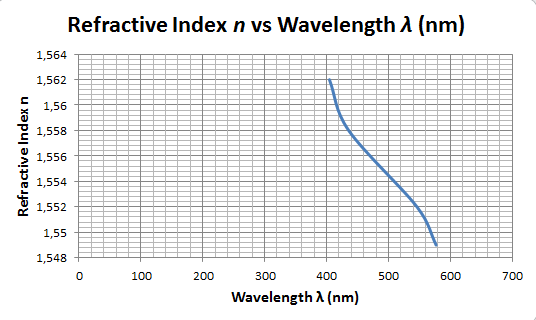
\includegraphics[width=1.0\linewidth, height=0.4\textheight]{graph1st}
\caption{Refractive Index n versus Wavelength $\lambda$ graph}
\label{fig:graph1st}
\end{figure}

\textbf{2. Assuming that Cauchy's equation gives the correct form of the relationship between \textit{n} and $\lambda$, calculate the least square straight line for n versus $1/\lambda^{2}$. Plot this line on a graph with \textit{n} as ordinates and $1/\lambda^{2}$ as abscissae. Show the experimental points on the graph. Write on the graph values \textit{A} and \textit{B}.}
\newpage
\begin{figure}[h]
\centering
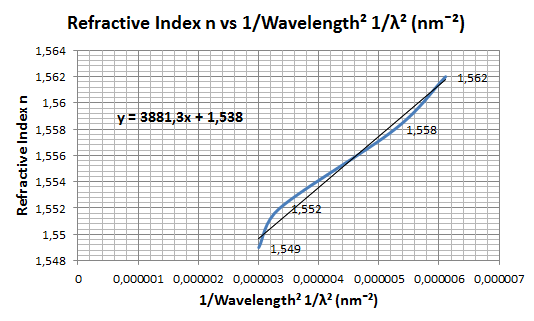
\includegraphics[width=1.0\linewidth, height=0.4\textheight]{graph2new}
\caption{Refractive Index n versus 1/Wavelength$^{2}$ $1/\lambda^{2}$ graph}
\label{fig:graph2new}
\end{figure}
As we can see from the graph, the graph equation is $y=3881.3x+1.538$. When we applied Cauchy's equation to the graph equation, A is equal to 1.538 and B is equal to 3881.3. When we solve the Cauchy's equation;
\begin{center}
	{\large $n=1.538+\frac{3881.3}{\lambda^{2}}$}   
\end{center}
By solving Cauchy's equation we show that the refraction index is depend on the wavelength.













\chapter{Discussion and Conclusion}
\textbf{1. What are the possible errors in the experiment?}\\
The first possible error cause was the calibration of the prism spectrometer. In our setup the calibration of the prism was almost certain.  The second error cause was location of the prism. Since incident ray refract from prism, location of the prism is important. In the experiment, we may had some errors. The third error cause was the reading of the Vernier Scale. It was the first time for us with using Vernier Scale. Since laboratory was dark and Vernier Scale was too small, it was very hard to read the corresponding points.\\ \\ 
\textbf{2. What kind of approximation did you take into consideration while you were obtaining the physical quantities and how do they affect your results?}\\
Approximations those are related to experiments were the reading Vernier Scale and spectrum of light. As we know all scales have their own errors. I mean, the smallest slit was 1 mm. Besides when we look through the eyepiece, making decisions about light spectrum also caused to experimental error.\\\\
\textbf{3. What discrepancies did you encounter between the calculated quantities and theoretical or literature values?}\\
Apperantly we do not have a certain discrepancies it is because our experimental error is too small. If we calculate our percentage error by using the following formula, we will see more clearly.

\begin{center}
	Percentage Error=$\frac{|Theoretical Value-Experimental Value|}{Theoretical Value}\times \% 100$

	Percentage Error=$\frac{|59.42-59.30|}{59.
		42}\times \% 100$

		Percentage Error = 0.2\%
\end{center}
\\
\textbf{4. What is your overall conclusion?}\\
We can see from the previous steps, we did experiment well. Light spectrum, wavelength and refraction index are studied well also.  
\chapter{Application}
\textbf{Spectrophotometry}\\\\
Spectrophotometry is a powerful tool for analyzing substances that have color such as aspirin transition metal ion complexes and
anions $[5]$. Principle of spectrophotometry is that every substance absorbs
or transmits certain wavelengths of radiant energy but not other wavelengths.
For example, chlorophyll always absorbs red and violet light, while it transmits
yellow, green, and blue wavelengths. The transmitted and reflected wavelengths
appear green—the color your eye “sees.” The light energy absorbed
or transmitted must match exactly the energy required to cause an electronic
transition (a movement of an electron from one quantum level to another) in
the substance under consideration. Only certain wavelength photons satisfy
this energy condition. Thus, the absorption or transmission of specific wavelengths
is characteristic for a substance, and a spectral analysis serves as a
“fingerprint” of the compound.
\begin{figure}[h]
\centering
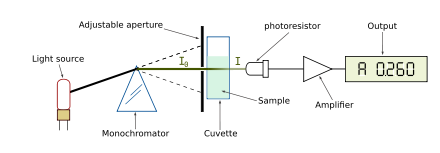
\includegraphics[width=0.90\linewidth, height=0.25\textheight]{Spectrophotometry}
\caption{Procedure of Spectrophotometry}
\label{fig:Spectrophotometry}
\end{figure}














\chapter{References}
$[1]$ Hecht, E. (2002). \textit{Optics} (4th ed., pp. 187-188). Reading, Mass.: Addison-Wesley.\\\\
$[2]$ Loshin, D. (1991). \textit{The Geometrical Optics Workbook} (pp. 49-50). Boston: Butterworth-Heinemann.\\\\
$[3]$ (n.d.). Retrieved March 12, 2015, from http://www.physics.nus.edu.sg\\/~L1000/PC1142/PrismSpectrometer.pdf\\\\
$[4]$ Chartier, G. (2005). \textit{Introduction to Optics} (p. 363). New York: Springer.\\\\
$[5]$ Beran, J. (2011). \textit{Laboratory Manual for Principles of General Chemistry} (9th ed., p. 376). Hoboken, NJ: Wiley.



























































































\end{document}          
